\section{Pilot: cross-simulator robustness}
\label{sec:pilot}

The pilot runs the twelve candidates at both sizes in six worlds: two ABIDES configurations (A1, the RMSC04 reference; A5, with more market making), two hand-set Hawkes regimes (H1 liquid, H2 thin), and MarS with the 10M and 2M models (M10, M2). Each world keeps its own conventions, so this is a comparison across domains, not a like-for-like one. In total \nPilotRows{} policy rollouts were attempted and \nPilotUsed{} are used.

\subsection{Stability comes first}

\begin{table}[!htbp]
\centering\footnotesize
\caption{Stability audit of the pilot. Volume pass: unperturbed runs used to size the parent order. Main pass: a seed fails if its burn-in or its unperturbed twin fails; it is screened out if the mid moved more than 200\,bps in the five minutes before the task. Last three columns describe the unperturbed twin over the ten-minute task in the seeds used: standard deviation of the mid move, share of seeds moving more than 3\%, and mean quoted spread.}\label{tab:audit}
\resizebox{\ifdim\width>\linewidth\linewidth\else\width\fi}{!}{%
\begin{tabular}{llrrrrrrrrr}
\toprule
World & Family & \multicolumn{2}{c}{Volume pass} & \multicolumn{4}{c}{Main pass (seeds)} & Move s.d. & $>$3\% & Spread \\
 & & run & failed & run & failed & screened & used & (bps) & & (bps) \\
\midrule
A1 & abides & 20 & 0 & 40 & 0 & 0 & 40 & 5 & 0\% & 0.2 \\
A5 & abides & 20 & 0 & 40 & 0 & 0 & 40 & 5 & 0\% & 0.1 \\
H1 & hawkes & 20 & 0 & 60 & 0 & 0 & 60 & 52 & 0\% & 11.7 \\
H2 & hawkes & 20 & 0 & 60 & 0 & 3 & 57 & 153 & 5\% & 20.2 \\
M10 & mars & 12 & 7 & 10 & 4 & 1 & 5 & 63 & 0\% & 14.6 \\
M2 & mars & 12 & 4 & 11 & 1 & 0 & 10 & 277 & 10\% & 21.7 \\
\bottomrule
\end{tabular}}
\end{table}


Table~\ref{tab:audit} is the audit that precedes any cost number. ABIDES and the Hawkes simulator completed every run. MarS did not. In the volume pass, \marsVolFail{} unperturbed rollouts (10M and 2M) failed: the burn-in or the rollout exceeded its time limit in a burst of order generation, the book emptied and the engine raised an error, or an internal assertion fired. In the main pass, \marsMainFail{} seeds were lost to failure or to the pre-task screen, and of the policy rollouts on the remaining seeds a further 15 of 120 (10M) and 13 of 240 (2M) failed. Because of the time limits, some of these are slow rollouts on a loaded machine, not crashes; all of them are runs that a practitioner would not obtain a number from. The surviving sample is therefore selected on stability, and it is small: five seeds for the 10M model.

Among surviving seeds the 2M model's unperturbed mid still moves by more than 3\% in ten minutes in 10\% of cases, with a standard deviation of 277\,bps, five times that of the liquid Hawkes regime and fifty times that of ABIDES.

\subsection{Costs and what each world recommends}

\begin{table}[!htbp]
\centering\footnotesize
\caption{Pilot: implementation shortfall in bps (mean $\pm$ 95\% half-width) for a parent order of 15\% of background volume. Bold: lowest mean in the column. Costs are not comparable across columns: the worlds have different price levels and tick sizes.}\label{tab:pilotcost15}
\resizebox{\ifdim\width>\linewidth\linewidth\else\width\fi}{!}{%
\begin{tabular}{lrrrrrr}
\toprule
Policy & A1 & A5 & H1 & H2 & M10 & M2 \\
\midrule
P0 TWAP & 0.4{\tiny$\,\pm$1.0} & 0.3{\tiny$\,\pm$0.9} & 39.0{\tiny$\,\pm$10.2} & 58.0{\tiny$\,\pm$28.2} & 257.2{\tiny$\,\pm$339.8} & 28.8{\tiny$\,\pm$28.4} \\
P1 Immediate & 1.7{\tiny$\,\pm$0.5} & 1.1{\tiny$\,\pm$0.3} & 43.8{\tiny$\,\pm$5.9} & 57.4{\tiny$\,\pm$16.5} & \textbf{38.9{\tiny$\,\pm$18.7}} & 34.5{\tiny$\,\pm$25.1} \\
P2 Front-loaded ($b{=}2$) & 0.5{\tiny$\,\pm$0.7} & 0.5{\tiny$\,\pm$0.6} & 45.9{\tiny$\,\pm$9.5} & 50.2{\tiny$\,\pm$20.4} & 778.6{\tiny$\,\pm$922.4} & 14.0{\tiny$\,\pm$26.3} \\
P2 Front-loaded ($b{=}4$) & 1.4{\tiny$\,\pm$1.3} & 0.7{\tiny$\,\pm$0.4} & 44.9{\tiny$\,\pm$9.2} & 54.1{\tiny$\,\pm$18.0} & 79.7{\tiny$\,\pm$45.9} & 3.5{\tiny$\,\pm$17.9} \\
P3 Back-loaded & 0.5{\tiny$\,\pm$1.2} & 0.3{\tiny$\,\pm$1.1} & 38.5{\tiny$\,\pm$11.9} & 69.9{\tiny$\,\pm$33.0} & 97.7{\tiny$\,\pm$85.8} & \textbf{0.0{\tiny$\,\pm$38.0}} \\
P4 POV ($1\times$) & 0.4{\tiny$\,\pm$0.8} & 0.3{\tiny$\,\pm$0.8} & 46.7{\tiny$\,\pm$11.9} & 68.2{\tiny$\,\pm$27.7} & 564.7{\tiny$\,\pm$348.2} & 5.5{\tiny$\,\pm$12.1} \\
P4 POV ($2\times$) & 1.1{\tiny$\,\pm$0.7} & 0.8{\tiny$\,\pm$0.5} & 45.1{\tiny$\,\pm$6.7} & 50.2{\tiny$\,\pm$21.4} & 411.7{\tiny$\,\pm$411.7} & 22.3{\tiny$\,\pm$27.0} \\
P5 Liquidity-aware & 0.5{\tiny$\,\pm$0.9} & 0.3{\tiny$\,\pm$0.9} & 36.8{\tiny$\,\pm$12.8} & 78.0{\tiny$\,\pm$27.5} & 209.8{\tiny$\,\pm$201.5} & 7.5{\tiny$\,\pm$19.1} \\
P6 Signal (momentum) & 0.7{\tiny$\,\pm$1.0} & 0.9{\tiny$\,\pm$1.0} & 40.0{\tiny$\,\pm$12.0} & 80.3{\tiny$\,\pm$28.1} & 42.0{\tiny$\,\pm$271.4} & 21.7{\tiny$\,\pm$28.1} \\
P6 Signal (reversal) & \textbf{0.3{\tiny$\,\pm$0.9}} & \textbf{-0.1{\tiny$\,\pm$0.9}} & 40.5{\tiny$\,\pm$10.5} & 63.7{\tiny$\,\pm$26.4} & 346.6{\tiny$\,\pm$457.9} & 20.7{\tiny$\,\pm$30.8} \\
P7 Risk-aware (0.5) & 3.4{\tiny$\,\pm$2.2} & 1.1{\tiny$\,\pm$0.4} & 38.0{\tiny$\,\pm$5.9} & 37.8{\tiny$\,\pm$18.7} & 258.1{\tiny$\,\pm$347.1} & 29.0{\tiny$\,\pm$33.4} \\
P7 Risk-aware (2) & 2.7{\tiny$\,\pm$0.9} & 1.4{\tiny$\,\pm$0.4} & \textbf{36.3{\tiny$\,\pm$5.3}} & \textbf{35.4{\tiny$\,\pm$19.3}} & 235.5{\tiny$\,\pm$278.3} & 15.6{\tiny$\,\pm$11.9} \\
\midrule
Seeds & 40 & 40 & 60 & 57 & 5 & 10 \\
Half-spread (bps) & 0.1 & 0.1 & 5.8 & 10.1 & 7.3 & 10.8 \\
\bottomrule
\end{tabular}}
\end{table}


Table~\ref{tab:pilotcost15} gives shortfall at 15\% of volume (5\% is in Appendix~\ref{app:pilot}). Three patterns matter.

\emph{ABIDES barely distinguishes the candidates.} All costs are below 4\,bps and most intervals overlap. Only the immediate order, the fast front-loaded schedule and the risk-aware controller are visibly dearer.

\emph{The Hawkes regimes price impact an order of magnitude higher}, at 35 to 80\,bps, and disagree with each other about adaptive rules: the liquidity-aware rule is among the best in the liquid regime and among the worst in the thin one.

\emph{MarS inverts the ordering, violently.} With the 10M model, TWAP costs 257\,bps and the immediate order 39\,bps at 15\% of volume; at 5\% the gap is 905 against 20\,bps. A persistent seller is met by a market that keeps falling (Figure~\ref{fig:intervention}), which is the behaviour already visible in the official example. With five usable seeds and intervals of hundreds of basis points these are anecdotes, but they are consistent in sign across sizes for the 10M model. The 2M model does not show the same ordering.

\begin{figure}[!htbp]
\centering
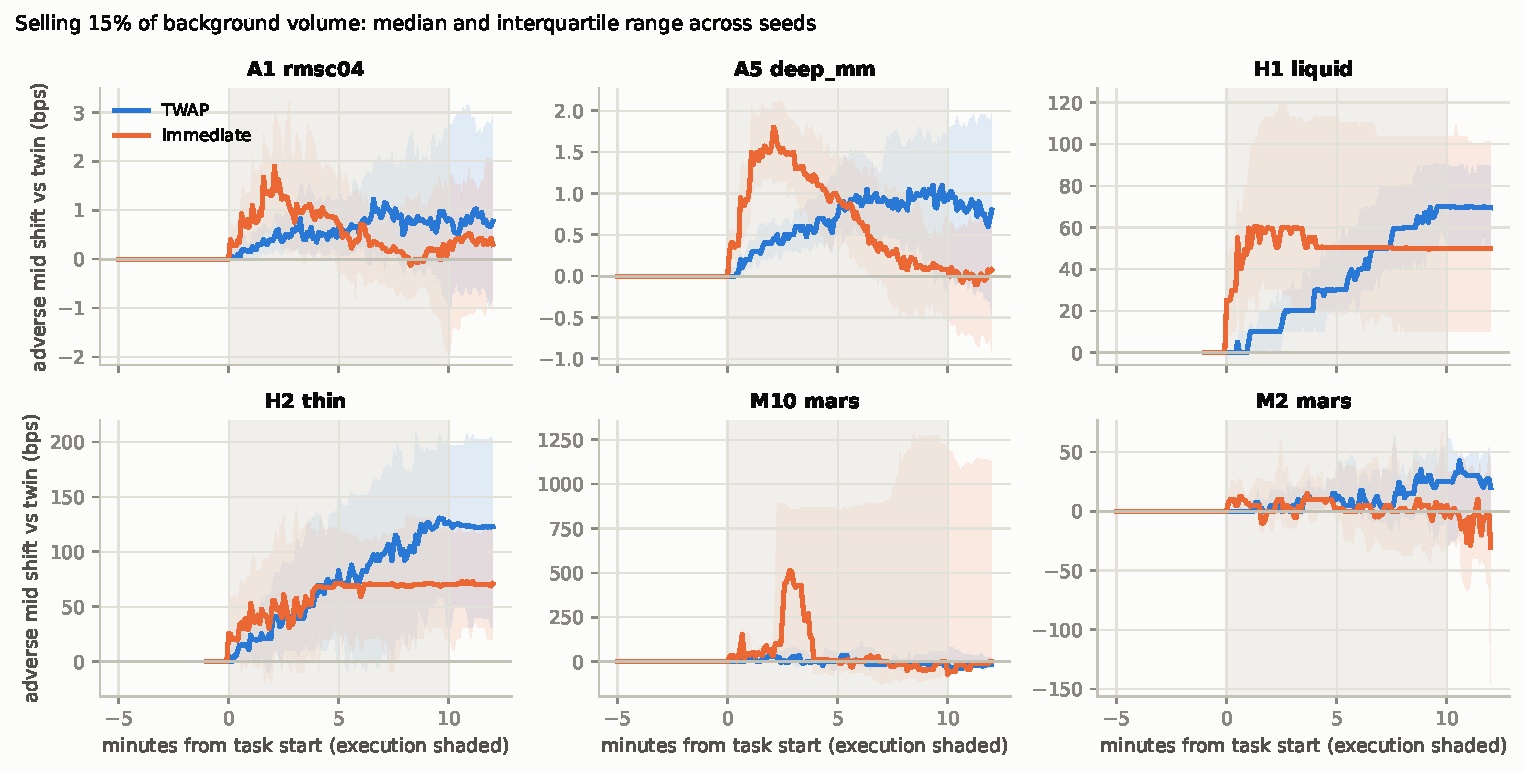
\includegraphics[width=\linewidth]{figures/fig_pilot_intervention.pdf}
\caption{Intervention against no intervention: adverse shift of the mid price relative to the unperturbed twin, for TWAP and immediate execution of 15\% of background volume. Lines are medians across seeds, bands the interquartile range. Vertical scales differ by three orders of magnitude.}
\label{fig:intervention}
\end{figure}

\subsection{Transfer between simulators}

Selecting each world's cheapest candidate on half its seeds and evaluating it on the other half of every world's seeds gives the cross-simulator matrix (Table~\ref{tab:cross} in the appendix, Figure~\ref{fig:pilotregret}). Policy rankings agree weakly within a family (mean Spearman correlation \rankSame{}) and not at all across families (\rankCross{}). Of the \nCross{} off-diagonal transfers, \nSigCross{} carry a regret whose interval lies above zero. The largest regrets, tens of half-spreads, arise when a policy chosen elsewhere is evaluated in MarS, or when a policy tuned to the Hawkes regimes is evaluated in ABIDES, whose half-spread is a tenth of a basis point.

\begin{figure}[!htbp]
\centering
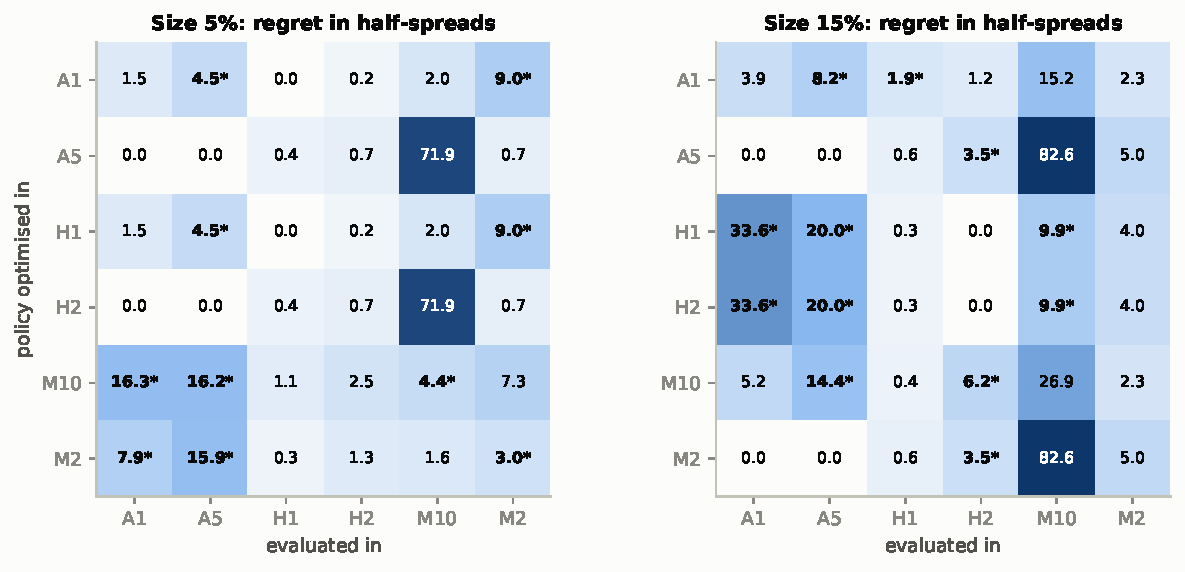
\includegraphics[width=0.85\linewidth]{figures/fig_pilot_regret.pdf}
\caption{Cross-simulator regret in units of the evaluation world's half-spread. An asterisk marks a paired 95\% interval above zero. Colour is on a square-root scale.}
\label{fig:pilotregret}
\end{figure}

This establishes that the simulators do not agree, and nothing more. The worlds differ in price level, tick, liquidity and calibration, and none of them is tied to a real market. Disagreement cannot say which, if any, is right. That needs a ground truth.

\section{Controlled decision validity}
\label{sec:reference}

\subsection{Design}

We wrote \nRefWorlds{} reference worlds from two mechanisms that are deliberately unlike any of the candidates (Table~\ref{tab:refworlds}, Appendix~\ref{app:worlds}): a queue-reactive book, where order flow depends only on the current queues, and a mix of behavioural traders (noise, fundamentalists, trend followers, and liquidity providers who withdraw from one-sided flow) with a hidden regime. Each candidate simulator receives \nFitEpisodes{} unperturbed 30-minute episodes from a reference world, as event logs and quotes, and nothing else. It is fitted to that data, then asked which of the twelve candidates it prefers at each size. Separately, every candidate policy is run in the reference world itself on \nRefSeeds{} seeds; half select the best-in-class policy and the other half measure regret.

\begin{table}[!htbp]
\centering\small
\caption{Reference worlds.}\label{tab:refworlds}
\resizebox{\ifdim\width>\linewidth\linewidth\else\width\fi}{!}{%
\begin{tabular}{ll}
\toprule
World & Mechanism and regime \\
\midrule
R1a & Queue-reactive, deep and resilient \\
R1b & Queue-reactive, thin, flow chases imbalance \\
R2a & Agent mix, strong fundamental anchor \\
R2b & Agent mix, trend followers dominate \\
\bottomrule
\end{tabular}}
\end{table}


The \emph{reference regret} of a simulator is the cost, in the reference world, of the policy it recommends minus the cost of the best candidate there. It is zero for a simulator that picks the best candidate and is bounded by the worst. It is a statement about these twelve policies in these four synthetic worlds.

\subsection{The truth being recovered}

\begin{table}[!htbp]
\centering\footnotesize
\caption{Reference worlds: the truth each simulator is judged against. Best: lowest-cost candidate on half the reference seeds; its cost and all regrets (bps) are measured on the other half. Sig.\ worse: candidates whose paired 95\% interval lies above the best. Raw and adjusted s.d.: per-seed standard deviation of shortfall before and after the control-variate adjustment.}\label{tab:reftruth}
\resizebox{\ifdim\width>\linewidth\linewidth\else\width\fi}{!}{%
\begin{tabular}{llrrrrlrrr}
\toprule
World & Size & Best & Cost & TWAP & Immediate & Worst candidate & Sig.\ worse & Raw s.d. & Adj.\ s.d. \\
\midrule
R1a & 5\% & POV $1\times$ & 5.1 & +0.0 & +0.0 & Front $b{=}4$ (+0.1) & 0 / 11 & 2 & 1 \\
R1a & 15\% & Momentum & 5.7 & -0.3 & +5.2 & Immediate (+5.2) & 1 / 11 & 3 & 2 \\
R1b & 5\% & Liquidity & 15.0 & +0.1 & +2.3 & Immediate (+2.3) & 0 / 11 & 26 & 16 \\
R1b & 15\% & Liquidity & 35.2 & -2.5 & +12.1 & Immediate (+12.1) & 1 / 11 & 30 & 21 \\
R2a & 5\% & Reversal & 3.0 & +3.0 & +12.4 & Immediate (+12.4) & 11 / 11 & 33 & 16 \\
R2a & 15\% & Reversal & 7.6 & +2.6 & +21.1 & Risk 2 (+22.9) & 11 / 11 & 33 & 17 \\
R2b & 5\% & Reversal & 5.0 & +3.1 & +11.4 & Risk 2 (+14.8) & 11 / 11 & 45 & 14 \\
R2b & 15\% & Reversal & 11.2 & +3.7 & +22.0 & Risk 2 (+24.5) & 11 / 11 & 44 & 14 \\
\bottomrule
\end{tabular}}
\end{table}


Table~\ref{tab:reftruth} shows that the worlds are not equally demanding. In the queue-reactive worlds the candidates are nearly interchangeable: only the immediate order is significantly worse than the rest, and only at the larger size. A recommendation can hardly go wrong there. The agent-mix worlds are discriminating. The reversal variant of the signal-aware rule is best in both regimes at both sizes, every other candidate is significantly worse, and the immediate order and the more risk-averse controller cost 21 to 25\,bps more at 15\% of volume. The reason is built into the mechanism: after an adverse move, fundamentalists push the price back, so waiting is rewarded.

\subsection{The fitted simulators}

\begin{table}[!htbp]
\centering\footnotesize
\caption{Fitted simulators in each reference world. Runs failed and moves above 3\%: unperturbed runs of the fitted simulator. A simulator is evaluated only if at most half fail and at most a quarter of the rest move more than 3\% in ten minutes. Realism error: mean scaled distance of six stylised facts from held-out reference data (lower is better; about 1 is within the reference world's own run-to-run variation). Volume ratio: simulator volume over reference volume.}\label{tab:refsims}
\resizebox{\ifdim\width>\linewidth\linewidth\else\width\fi}{!}{%
\begin{tabular}{llrrlrr}
\toprule
World & Simulator & Runs failed & Moves $>$3\% & Evaluated & Realism error & Volume ratio \\
\midrule
R1a & Hawkes & 0\% & 0\% & yes & 1.72 & 0.99 \\
R1a & ABIDES & 0\% & 0\% & yes & 10.63 & 0.96 \\
R1a & MarS & 33\% & 50\% & \textbf{no} & -- & 3.67 \\
R1b & Hawkes & 0\% & 0\% & yes & 0.21 & 0.97 \\
R1b & ABIDES & 0\% & 0\% & yes & 1.16 & 0.54 \\
R1b & MarS & 17\% & 40\% & \textbf{no} & -- & 1.88 \\
R2a & Hawkes & 0\% & 5\% & yes & 0.29 & 0.82 \\
R2a & ABIDES & 0\% & 0\% & yes & 0.79 & 0.40 \\
R2a & MarS & 33\% & 50\% & \textbf{no} & -- & 3.26 \\
R2b & Hawkes & 0\% & 0\% & yes & 0.60 & 1.21 \\
R2b & ABIDES & 0\% & 8\% & yes & 0.58 & 0.28 \\
R2b & MarS & 33\% & 50\% & \textbf{no} & -- & 1.79 \\
\bottomrule
\end{tabular}}
\end{table}


\paragraph{Hawkes.} The fit attributes much of the agent-mix worlds' order clustering to self-excitation: the estimated branching ratio is 0.34 and 0.47 in the queue-reactive worlds and 0.75 and 0.84 in the agent-mix worlds. Its unperturbed output is close to the reference on the realism score in three worlds (0.21, 0.29 and 0.60) and within about two units in the fourth.

\paragraph{ABIDES.} The grid search chose 180 value traders in three worlds and 102 in the fourth, with market makers in two. It matches the reference less well (1.16, 0.79, 0.58 and, in the deep queue-reactive world, 10.6, where ABIDES is far too volatile), and its traded volume is 28\% to 96\% of the reference's.

\paragraph{MarS.} Conditioned on replayed reference order flow, MarS did not produce a usable market in any world. Between 17\% and 33\% of its unperturbed runs failed, and of the rest 40\% to 50\% moved by more than 3\% within ten minutes, with traded volume two to four times the reference's. Under the screen in Table~\ref{tab:refsims} it was not asked for a recommendation. This is a statement about a pretrained model placed, without fitting, into a market unlike its training data; it is not a test of the MarS approach.

\subsection{Reference regret}

\begin{table}[!htbp]
\centering\footnotesize
\caption{Reference regret of each fitted simulator's recommendation (bps; $^\dagger$interval above zero). Tied: number of candidates the simulator cannot distinguish from its favourite; Worst tied: the largest reference regret among them. Rank $\rho$: Spearman correlation between the simulator's ranking of the twelve candidates and the reference world's.}\label{tab:refregret}
\resizebox{\ifdim\width>\linewidth\linewidth\else\width\fi}{!}{%
\begin{tabular}{lllllrrrrrr}
\toprule
World & Size & Simulator & Recommends & Ref.\ best & Regret & 95\% CI & Tied & Worst tied & Rank $\rho$ & Realism \\
\midrule
R1a & 5\% & Hawkes & Immediate & POV $1\times$ & +0.0 & [-0.2, 0.3] & 12 & +0.1 & 0.13 & 1.72 \\
R1a & 5\% & ABIDES & Momentum & POV $1\times$ & +0.1 & [-0.1, 0.3] & 4 & +0.1 & 0.02 & 10.63 \\
R1a & 15\% & Hawkes & Liquidity & Momentum & -0.1 & [-0.3, 0.0] & 5 & +0.0 & 0.50 & 1.72 \\
R1a & 15\% & ABIDES & Momentum & Momentum & +0.0 & [0.0, 0.0] & 2 & +0.0 & 0.55 & 10.63 \\
\addlinespace
R1b & 5\% & Hawkes & Back & Liquidity & -2.5 & [-5.8, 0.8] & 12 & +2.3 & 0.71 & 0.21 \\
R1b & 5\% & ABIDES & Momentum & Liquidity & +0.8 & [-2.7, 4.5] & 2 & +0.8 & 0.10 & 1.16 \\
R1b & 15\% & Hawkes & Risk 2 & Liquidity & -2.2 & [-5.7, 1.5] & 6 & +1.8 & 0.59 & 0.21 \\
R1b & 15\% & ABIDES & Liquidity & Liquidity & +0.0 & [0.0, 0.0] & 2 & +0.0 & 0.60 & 1.16 \\
\addlinespace
R2a & 5\% & Hawkes & Liquidity & Reversal & +4.0$^\dagger$ & [2.7, 5.5] & 3 & +4.0 & 0.66 & 0.29 \\
R2a & 5\% & ABIDES & Momentum & Reversal & +5.3$^\dagger$ & [3.8, 7.0] & 2 & +5.3 & 0.43 & 0.79 \\
R2a & 15\% & Hawkes & Immediate & Reversal & +21.1$^\dagger$ & [17.5, 25.0] & 7 & +22.9 & 0.04 & 0.29 \\
R2a & 15\% & ABIDES & Liquidity & Reversal & +1.8$^\dagger$ & [0.7, 2.9] & 2 & +3.8 & 0.69 & 0.79 \\
\addlinespace
R2b & 5\% & Hawkes & Immediate & Reversal & +11.4$^\dagger$ & [8.5, 14.2] & 4 & +11.4 & -0.13 & 0.60 \\
R2b & 5\% & ABIDES & Liquidity & Reversal & +6.1$^\dagger$ & [3.6, 9.1] & 8 & +9.0 & 0.65 & 0.58 \\
R2b & 15\% & Hawkes & Immediate & Reversal & +22.0$^\dagger$ & [18.0, 26.7] & 4 & +24.5 & -0.84 & 0.60 \\
R2b & 15\% & ABIDES & Momentum & Reversal & +4.9$^\dagger$ & [2.9, 7.0] & 3 & +4.9 & 0.85 & 0.58 \\
\bottomrule
\end{tabular}}
\end{table}


\begin{figure}[!htbp]
\centering
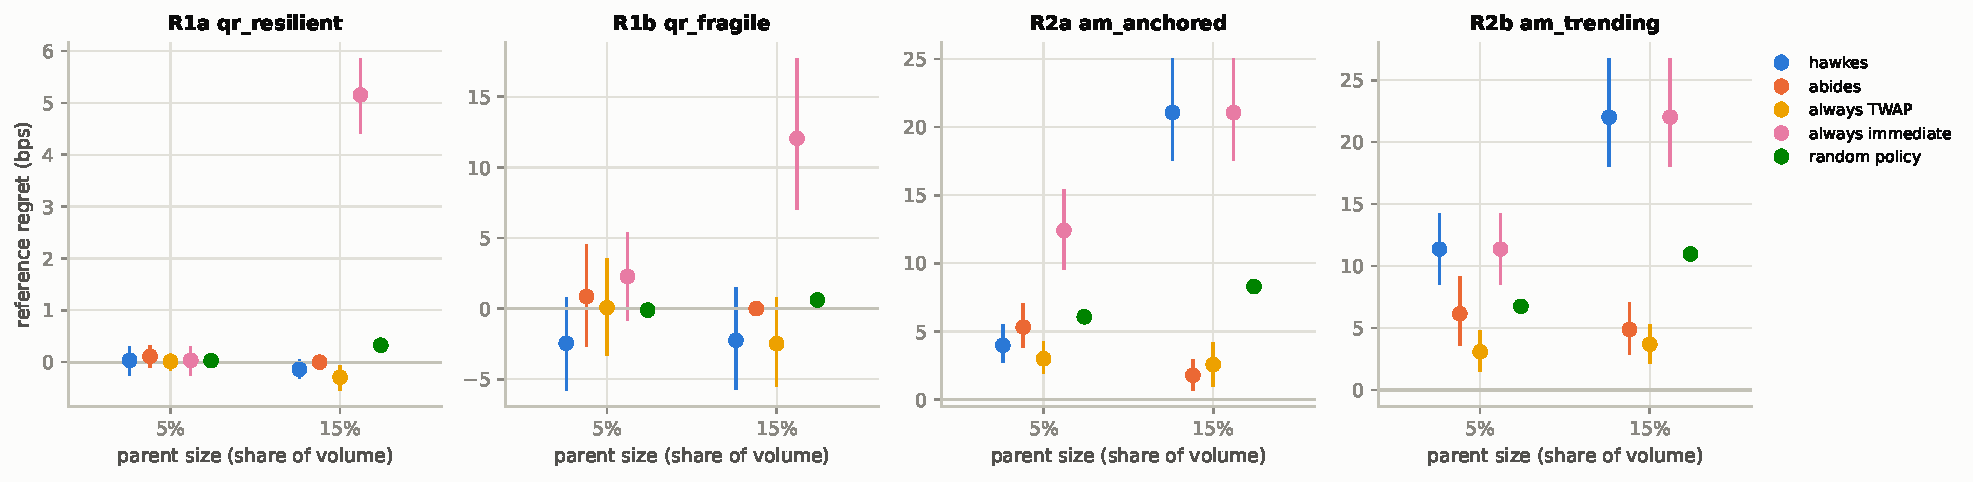
\includegraphics[width=\linewidth]{figures/fig_reference_regret.pdf}
\caption{Reference regret of each recommender with 95\% intervals. ``Random policy'' is the mean regret over the twelve candidates.}
\label{fig:refregret}
\end{figure}

Table~\ref{tab:refregret} and Figure~\ref{fig:refregret} give the main result, and Table~\ref{tab:refsummary} summarises it.

\begin{table}[!htbp]
\centering\small
\caption{Reference regret by recommender, over all reference worlds and sizes in which it was evaluated. The last four rows are simulator-free baselines.}\label{tab:refsummary}
\resizebox{\ifdim\width>\linewidth\linewidth\else\width\fi}{!}{%
\begin{tabular}{lrrrrr}
\toprule
Recommender & Settings & Mean regret (bps) & Mean (half-spreads) & Max (half-spreads) & Sig.\ worse than best \\
\midrule
Hawkes & 8 & 6.7 & 1.10 & 3.60 & 4 \\
Hawkes (linear) & 8 & 4.9 & 0.79 & 3.99 & 4 \\
Hawkes (sqrt) & 8 & 4.9 & 0.81 & 3.60 & 3 \\
ABIDES & 8 & 2.4 & 0.40 & 1.00 & 4 \\
Always TWAP & 8 & 1.2 & 0.19 & 0.60 & 4 \\
Always immediate & 8 & 10.8 & 1.87 & 3.60 & 6 \\
Random candidate & 8 & 4.1 & 0.69 & 1.79 & 0 \\
Worst candidate & 8 & 11.8 & 2.03 & 3.99 & 0 \\
\bottomrule
\end{tabular}}
\end{table}


\emph{Neither fitted simulator beats the simplest rule.} Averaged over the eight settings, always choosing TWAP has a regret of 1.2\,bps. The ABIDES fits average 2.4\,bps, a uniformly random candidate 4.1\,bps, the Hawkes fits 6.7\,bps, and always choosing the immediate order 10.8\,bps, against 11.8\,bps for the worst candidate in each setting.

\emph{The simulator with the better realism score made the worst decisions.} In the anchored agent-mix world the Hawkes fit has a realism error of 0.29 against 0.79 for ABIDES. At 15\% of volume it recommends the immediate order, at a regret of 21.1\,bps (interval 17.5 to 25.0), close to the worst available; ABIDES recommends the liquidity-aware rule, at 1.8\,bps. In the trending world the two realism scores are within 0.03 of each other, and Hawkes again recommends the immediate order at both sizes (11.4 and 22.0\,bps) while ABIDES is at 6.2 and 4.9\,bps. Of the eight head-to-head comparisons between the two simulators' recommendations, four are statistically distinguishable: one small one favours Hawkes (1.3\,bps) and three favour ABIDES (5.2, 17.1 and 19.3\,bps).

\emph{Realism did not predict regret.} Across the \refPoints{} simulator--world--size points the Spearman correlation between realism error and regret is \refRho{} (permutation $p=\refRhoP{}$, shuffling realism scores among simulators within a world). With two simulators and four worlds this is descriptive, and the sign of a correlation this weak carries no information. The informative fact is the counterexample above.

\emph{Cost levels are not predicted either.} The Hawkes fits overstate costs by 53 and 71\,bps on average in the two agent-mix worlds at the larger size; the ABIDES fits overstate them by 8 and 67\,bps. More telling is the sign of one comparison. In both agent-mix worlds the immediate order truly costs about 18\,bps more than TWAP at 15\% of volume. ABIDES predicts $+10$ and $+54$\,bps. Hawkes predicts $-9$ and $-50$\,bps: it believes splitting the order is the expensive choice.

\subsection{Why the Hawkes fit fails, and an ablation}

A Hawkes process explains clustered flow by letting events trigger further events. Fitted to the agent-mix worlds it finds a branching ratio near 0.8, so in its world each child order of a sliced schedule sets off its own cascade of selling and cancellations, and twenty child orders set off twenty. In the reference world the clustering has a different cause, traders reacting to prices, and part of that reaction pushes the price back. Both accounts fit the unperturbed data. They disagree about what happens when someone intervenes, which is the only thing an execution study asks.

The same point can be made inside the Hawkes family. How strongly a market order excites later flow as a function of its size is an assumption of the simulator: unperturbed data contain few orders of the size of a parent order, so they barely constrain it. Table~\ref{tab:hawkesvariants} fits three versions (excitation linear in size up to ten mean order sizes; linear without an effective cap; square-root) to the same data.

\begin{table}[!htbp]
\centering\footnotesize
\caption{Three Hawkes simulators that differ only in how strongly a market order excites later flow as a function of its size, each fitted to the same reference data. Entries: recommended policy and its reference regret in bps ($^\dagger$interval above zero).}\label{tab:hawkesvariants}
\resizebox{\ifdim\width>\linewidth\linewidth\else\width\fi}{!}{%
\begin{tabular}{llrrr}
\toprule
World & Size & Capped linear & Linear & Square-root \\
\midrule
R1a & 5\% & Immediate (+0.0) & Immediate (+0.0) & Immediate (+0.0) \\
R1a & 15\% & Liquidity (-0.1) & Liquidity (-0.1) & Liquidity (-0.1) \\
R1b & 5\% & Back (-2.5) & Back (-2.5) & Reversal (-2.2) \\
R1b & 15\% & Risk 2 (-2.2) & Liquidity (+0.0) & Risk 2 (-2.2) \\
R2a & 5\% & Liquidity (+4.0$^\dagger$) & Liquidity (+4.0$^\dagger$) & Reversal (+0.0) \\
R2a & 15\% & Immediate (+21.1$^\dagger$) & Liquidity (+1.8$^\dagger$) & Immediate (+21.1$^\dagger$) \\
R2b & 5\% & Immediate (+11.4$^\dagger$) & Immediate (+11.4$^\dagger$) & Immediate (+11.4$^\dagger$) \\
R2b & 15\% & Immediate (+22.0$^\dagger$) & Risk 2 (+24.5$^\dagger$) & Front $b{=}4$ (+11.6$^\dagger$) \\
\midrule
\multicolumn{2}{l}{Mean realism error} & 0.71 & 0.71 & 0.76 \\
\bottomrule
\end{tabular}}
\end{table}


Their realism scores are almost identical. Their recommendations are not: in the anchored world at 15\% of volume the regret is 21.1, 1.8 and 21.1\,bps; in the trending world it is 22.0, 24.5 and 11.6\,bps. A choice that the realism score cannot see moves the decision from near-best to near-worst. None of the three does better on average than a random candidate.

\section{Discussion}

\paragraph{What the evidence supports.} In this controlled setting, observational realism was not a guide to decision validity. A simulator that reproduced the reference market's stylised facts well recommended one of the worst policies, a less realistic one did better, and three simulators with the same realism score recommended different policies. The mechanism is not exotic: two models can fit the same unperturbed data and differ in what they imply about interventions, and a realism score computed on unperturbed data cannot separate them.

\paragraph{What it does not support.} It does not show that agent-based simulators give better decisions than statistical ones. ABIDES did better than Hawkes here, in two reference worlds built from behavioural agents, which resemble ABIDES more than they resemble a Hawkes process; with other reference worlds the order could reverse. It does not show that realism is irrelevant, only that the score we used did not predict regret in sixteen points. And it says nothing about real markets.

\paragraph{The baseline result.} That TWAP beat both fitted simulators is partly a property of our reference worlds, in which the cost surface is flat near TWAP. It is still a useful discipline: a simulator-derived recommendation should be reported against simulator-free baselines, because a simulator can do worse than not using one.

\paragraph{Stability is a gate, not a detail.} MarS never reached the starting line in the controlled experiment and lost half its seeds in the pilot. We do not conclude that generative order-flow models are unfit for execution studies. We conclude that the released small models, started from the states available to us and run for tens of minutes, do not hold a market steady, and that their sensitivity to persistent flow, in which a patient seller moves the price by percent, should be checked before any cost estimate from them is used.

\section{Limitations}
\label{sec:limits}

\begin{itemize}[leftmargin=*,itemsep=2pt]
\item \textbf{No real data.} Realism against held-out historical data (the planned first experiment) was not measured, and no simulator was calibrated to a real instrument. All regret is inside simulated markets.
\item \textbf{The reference worlds are ours.} Two mechanisms, two regimes each. ``Best'' means best of twelve candidates. Two of the four worlds barely discriminate between policies.
\item \textbf{Unequal fits.} Hawkes shares the reference worlds' matching engine, lot and event vocabulary and is fitted by maximum likelihood on their event logs; ABIDES uses its own exchange and a three-parameter grid search; MarS could not be fitted at all.
\item \textbf{A thin realism score.} Six statistics of a 5-second quote grid. It ignores order sizes, event mix, depth and inter-arrival times. A richer score, in particular one that includes responses to large natural orders, might have flagged the Hawkes fit. We did not test that.
\item \textbf{MarS.} Small released models only; run on CPU outside the supported environment; trained on another market; initialised from synthetic states; child orders capped at visible depth; wall-clock limits contribute to its failure counts; surviving seeds are selected on stability and few.
\item \textbf{Pilot comparability.} Three matching engines, different price levels and ticks. Cross-simulator regret in the pilot is exploratory.
\item \textbf{Policies.} Market orders only; no limit orders, fees or latency; the optional MFG-derived policy was not included.
\item \textbf{Selection noise.} A recommendation is the candidate with the lowest mean cost over a simulator's seeds (100 for Hawkes, 30 for ABIDES). Where candidates are tied in the simulator, the choice is partly chance; Table~\ref{tab:refregret} reports the size of each tied set and the worst regret within it.
\item \textbf{Post-hoc choices.} The stability screen for fitted simulators, the floor in the realism score, the ABIDES grid and the Hawkes ablation were fixed after seeing early results. No analysis was pre-registered.
\end{itemize}

\section{Conclusion}

We asked whether a market simulator that looks realistic gives reliable execution decisions. Without real order-level data we could not ask it of real markets. Asked of markets whose rules we know, the answer in our experiment was no: the best-fitting simulator recommended a policy more than 20\,bps worse than the best available, a cruder fit did better, a pretrained generative model could not be stabilised at all, and none improved on always choosing TWAP. The reason is that fit to unperturbed data leaves the response to intervention undetermined. Simulator validation for execution should therefore include what realism scores omit: stability without intervention, behaviour under interventions of the size to be studied, and comparison with simulator-free baselines.
